\documentclass[conference]{IEEEtran}

\usepackage{graphicx} % Required for inserting images
\usepackage{geometry}
\usepackage{minted}
\usepackage{hyperref}
\usepackage{mathtools}
\usepackage{enumitem}
\usepackage{amssymb}
\usepackage{float}

\DeclareMathOperator{\dom}{dom}
\geometry{letterpaper, margin = 1in}

\def\BibTeX{{\rm B\kern-.05em{\sc i\kern-.025em b}\kern-.08em
    T\kern-.1667em\lower.7ex\hbox{E}\kern-.125emX}}


\begin{document}
\title{
Subgradient Methods Applied to LASSO Regression
}

\author{\IEEEauthorblockN{Kasey Tian}
\IEEEauthorblockA{\textit{Electrical and Computer Engineering} \\
\textit{Rutgers University}\\
New Brunswick, NJ, USA \\
kasey.tian@rutgers.edu}
}


\maketitle

\begin{abstract}
Subgradient methods
\end{abstract}

\begin{IEEEkeywords}
optimization, subgradients, LASSO, regression
\end{IEEEkeywords}

\section{Introduction}\label{sec:intro}
Subgradient methods are a way to perform an optimization on an objective function which is not fully differentiable. For non-differentiable objective functions, traditional methods, such as gradient descent and Newton's method, are impossible to execute. They can also be combined with a wide variety of other optimization methods, and have far reaching applications. They were originally developed by Shor and others in the Soviet Union in the 1960s and 70s \cite{boydparksubgradients}.


\section{Mathematical Basis}\label{sec:math}
In this section we will explore the mathematics of subgradient methods and the LASSO Regression method.
\subsection{Subgradient}\label{sec:math subgrad}
\subsubsection{Definitions}
A subgradient is defined for some convex function \(f: \mathbb{R}^n \rightarrow \mathbb{R}\) at a point \(x \in \dom f\) as a vector \(g \in \mathbb{R}^n\) such that \(\forall y \in \dom f\)
\begin{equation}\label{eq:subgradient def}
f(y) \geq f(x) + g^T (y-x) 
\end{equation}
There can be multiple subgradients at a point \(x\), so we will also define the subdifferential \(\partial f(x)\) to be the set of all subgradients at \(x\).
\begin{equation}\label{eq:math subdifferential}
\partial f(x) = \left\{ g : f(y) \geq f(x) + g^T (y-x)\right\}
\end{equation}

\subsubsection{Example: Absolute Value}
If we consider \(g\) in \eqref{eq:subgradient def} to be a slope, we can visualize a subgradient as being some hyperplane intersecting our function at \(x\) for which all values of the function are on or above the plane. 

Let us employ this intuition to find a subgradient of the function \(f(x) = |x|\) at the point \(x=0\). Graphically, we can see in Fig. \ref{fig:abs subgradients} that many different lines satisfy this criteron.
\begin{figure}[tbp]
    \centering
    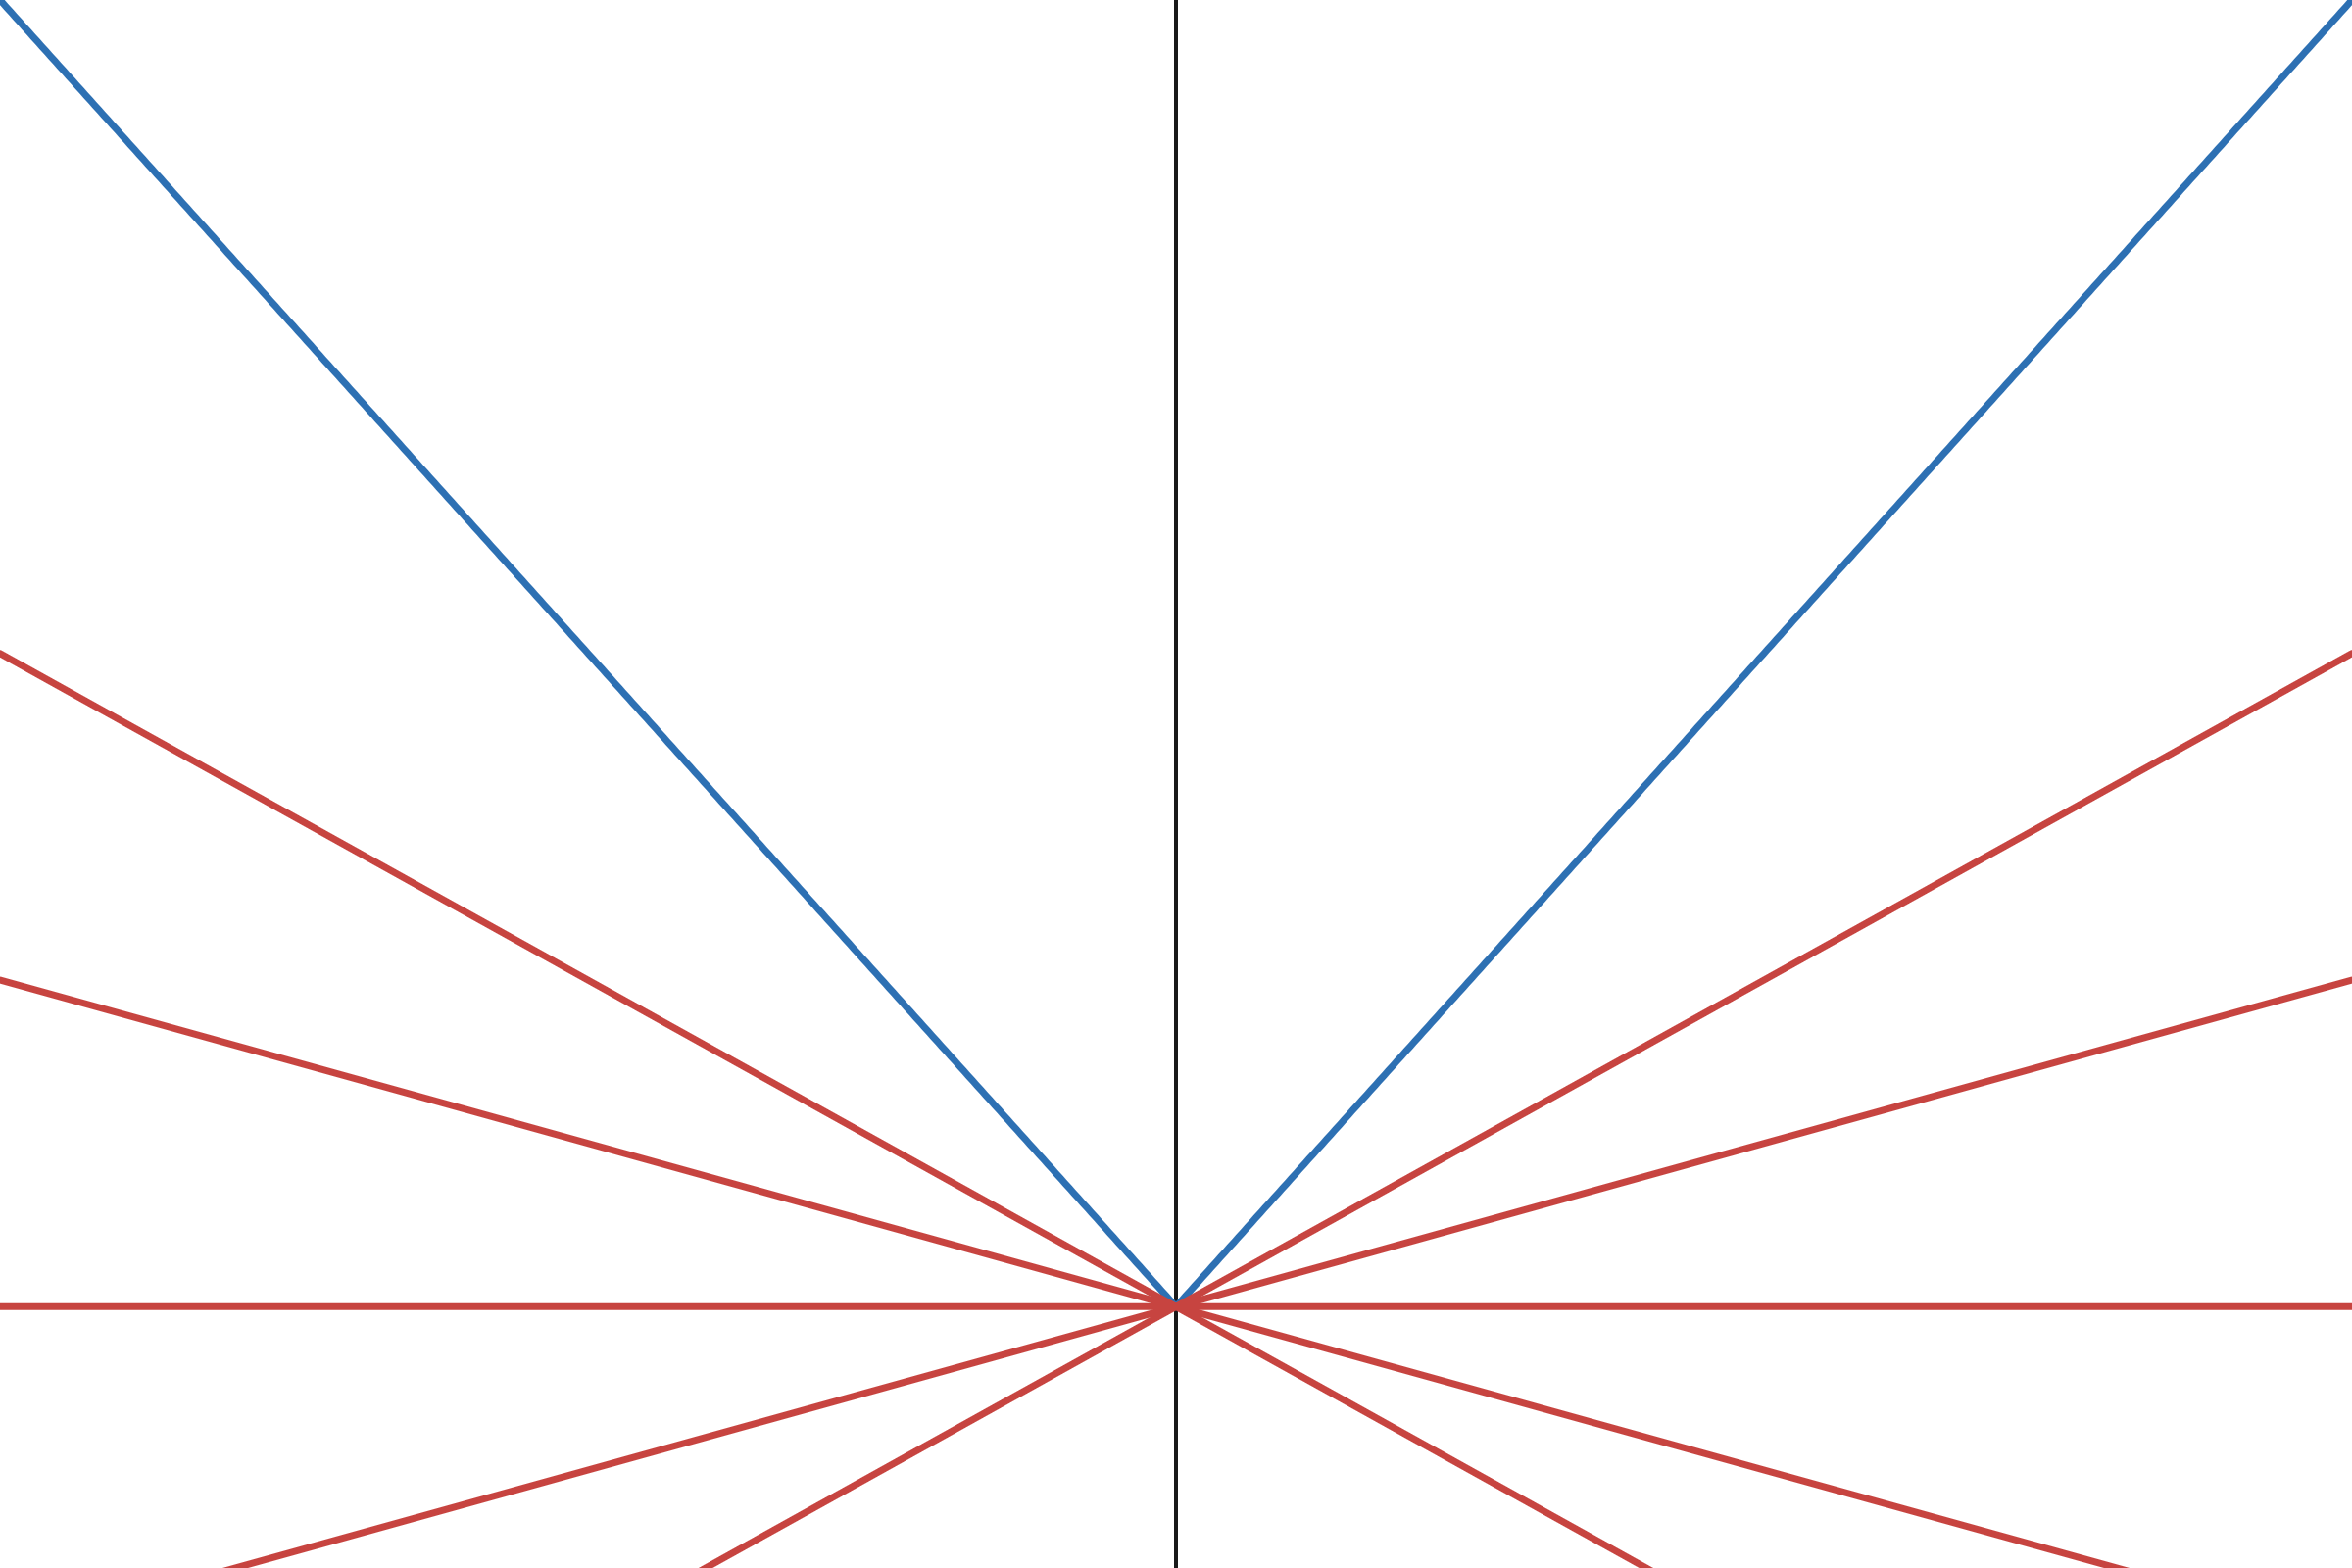
\includegraphics[width=0.9\linewidth]{Figures/abs_subgradients.png}
    \caption{Subgradients of absolute value function.}
    \label{fig:abs subgradients}
\end{figure}
In fact, we can say that any \(g \in [-1,1]\) would be a subgradient, and therefore \(\partial f(0) = [-1,1]\). But what about other points? For a point \(x > 0\), we can surmise that the only possible \(g = 1\), as any other value will leave some parts of our function beneath the resulting plane. Likewise for \(x < 0\), \(g = -1\). Thus we can write
\begin{equation}\label{eq:abs subdifferential}
\partial f(x) = \begin{cases}
    -1 & x < 0 \\
    [-1, 1] & x = 0\\
    1 & x > 0
\end{cases}
\end{equation}
This can be compared against the derivative of \(f(x)\).
\begin{equation}\label{eq:abs derivative}
f'(x) = \begin{cases}
            -1 & x < 0\\
            1 & x > 0
\end{cases}
\end{equation}
We find that where the function is differentiable, the subdifferential contains only the gradient. There is only a difference where the function is not differentiable.

\subsubsection{Properties}
There are a few important properties that we shall take note of. Proofs of these properties can be found in Appendix \ref{sec:subgradient properties proofs}.
\begin{enumerate}
    \item If the function is differentiable at \(x\), the only member of \(\partial f(x)\) will be the gradient
    \item If \(x\) is a global minimum, \(\partial f(x)\) must contain the zero vector
\end{enumerate}


\subsection{LASSO Regression}\label{sec:math lasso}

\section{Code Implementation}\label{sec:code}

\section{Numerical Results}\label{sec:results}

\section{Conclusion}\label{sec:conclusion}

\appendix
\subsection{Subgradient Properties}\label{sec:subgradient properties proofs}
\subsubsection{}

\subsection{Second Appendix}
ha ha ha

\bibliographystyle{IEEEtran}
\bibliography{refs}

\end{document}